\documentclass[a4j,12pt,]{jarticle}
 \usepackage[dvipdfmx]{graphicx}
 \usepackage{float}
 \usepackage{siunitx} %%SI単位系用
 \usepackage{amssymb, amsmath}
 \usepackage{ascmac,here,txfonts,txfonts}
\usepackage{listings,jlisting}
\usepackage[dvipdfmx]{color}
\lstset{%
  language={Python},
  basicstyle={\small},%
  identifierstyle={\small},%
  commentstyle={\small\itshape\color[rgb]{0,0.5,0}},%
  keywordstyle={\small\bfseries\color[rgb]{0,0,1}},%
  ndkeywordstyle={\small},%
  stringstyle={\small\ttfamily\color[rgb]{1,0,1}},
  frame={tb},
  breaklines=true,
  columns=[l]{fullflexible},%
  numbers=left,%
  xrightmargin=0zw,%
  xleftmargin=3zw,%
  numberstyle={\scriptsize},%
  stepnumber=1,
  numbersep=1zw,%
  lineskip=-0.5ex%
}
\begin{document}

{\noindent\small 第12回報告書 \hfill\today}
\begin{center}
  {\Large 分布定数線路の伝達関数について}
\end{center}
\begin{flushright}
  愛媛大学工学部 \\
  8531037m \\
  祖父江匠真 \\
\end{flushright}

\section{はじめに}

分布定数線路のF行列を用いて, 伝達関数を求めた.

\section{分布定数線路の伝達関数の導出}

分布定数回路のF行列

\[
  \left(
  \begin{array}{cc}
      A & B \\
      C & D
    \end{array}
  \right) =
  \left(
  \begin{array}{cc}
      \cosh\gamma l             & Z_0\sinh\gamma l \\
      \frac{\sinh\gamma l}{Z_0} & \cosh\gamma l
    \end{array}
  \right)
\]

のFパラメータを, 図 \ref{p1}で求めた


\begin{eqnarray}
  F =  \frac{1}{A + \frac{B}{R_2} + R_1C + \frac{R_1}{R_2}D}
\end{eqnarray}

に代入することで, 分布定数線路に抵抗$R_1$, 抵抗$R_2$を接続したときの回路における伝達関数Fを求める.

\begin{figure}[H]
  \begin{center}
    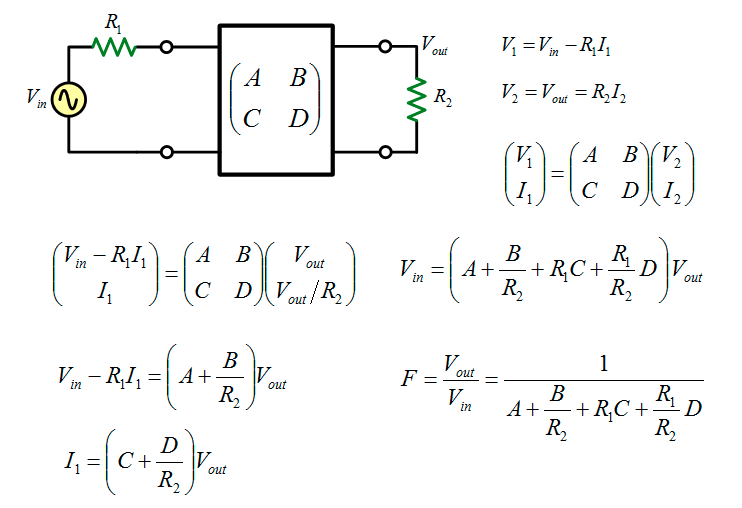
\includegraphics[width=140mm]{p1.png}
    \caption{伝達関数の導出過程}
    \label{p1}
  \end{center}
\end{figure}

図 \ref{p2}の回路図について, 伝達関数を求める.

\begin{figure}[H]
  \begin{center}
    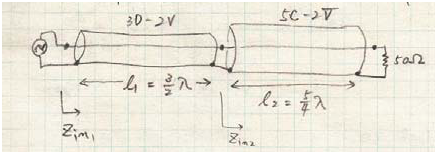
\includegraphics[width=140mm]{p2.png}
    \caption{回路図}
    \label{p2}
  \end{center}
\end{figure}

Pythonで伝達関数を計算するプログラムをソースコード \ref{sc1}に示す.

\begin{lstlisting}[caption=伝達関数の計算,label=sc1]
  import numpy as np

  def calculateTheta(cableLength, alpha):
      """
      伝搬定数γと同軸ケーブルの長さlの積を求める
      """
      beta = 2 * np.pi
      gamma = alpha + beta * 1j
      return gamma * cableLength
  
  
  def createFMatrixForDcc(Z0, theta):
      """
      分布定数回路のF行列を求める
      """
      return np.array(
          [
              [np.cosh(theta), Z0 * np.sinh(theta)],
              [np.sinh(theta) / Z0, np.cosh(theta)],
          ]
      )
  
  
  def calculateInputImpedanceByFMatrix(
    Z0,
    Zr,
    cableLength,
    alpha=0,
  ):
      """
      受電端に抵抗を接続した分布定数回路の入力インピーダンスを求める
      """
      theta = calculateTheta(cableLength, alpha)
  
      # 分布定数回路のF行列
      f_matrix_dcc = createFMatrixForDcc(Z0, theta)
  
      # 受電端のZrのF行列
      f_matrix_Zr = np.array(
          [
              [1, 0],
              [1 / Zr, 1],
          ]
      )
  
      # 受信端にZrを接続した場合のf行列
      f_matrix = np.dot(f_matrix_dcc, f_matrix_Zr)
  
      return abs(f_matrix[0, 0] / f_matrix[1, 0])
  
  
  def createTransferFunction(Z0, Zr, cableLength, alpha=0):
      """
      受電端に抵抗を接続した分布定数回路の伝達関数を求める
      """
      R1 = 0  # 入力側の抵抗は0で考える
      R2 = Zr
  
      theta = calculateTheta(cableLength, alpha)
      f_matrix_dcc = createFMatrixForDcc(Z0, theta)

      # Fパラメータを取り出す
      A = f_matrix_dcc[0][0]
      B = f_matrix_dcc[0][1]
      C = f_matrix_dcc[1][0]
      D = f_matrix_dcc[1][1]
  
      # 伝達関数
      return 1 / (A + B / R2 + R1 * C + (R1 / R2) * D)
  
  
  # 5C-2V
  l2 = 5 / 4
  Z02 = 75  # 同軸ケーブルのインピーダンス
  alpha2 = 7.6
  Zr = 50  # 受端のインピーダンス
  
  # 3D-2V
  l1 = 3 / 2
  Z01 = 50  # 同軸ケーブルのインピーダンス
  alpha1 = 13
  
  # 5C-2V + Zrの回路の入力インピーダンスを求める
  Zin2 = calculateInputImpedanceByFMatrix(Z02, Zr, l2, alpha2)
  
  # 伝達関数を求める
  transferFunc2 = createTransferFunction(Z02, Zr, l2, alpha2)
  transferFunc1 = createTransferFunction(
      Z01, Zin2, l1, alpha1
  )  #  5C-2V + Zrの回路の入力インピーダンスを受電端側の抵抗とする
\end{lstlisting}

\section{おわりに}

今回は分布定数線路のF行列から伝達関数を求めた.
次回は求めた伝達関数を用いて減衰の確認を行う.

\begin{thebibliography}{5}
  \bibitem{1}株式会社マクニカ,”縦続行列-半導体事業-マクニカ”,https://www.macnica.co.jp/business/semiconductor/articles/basic/127625,参照 November 24,2021.
\end{thebibliography}

\end{document}